\section{Introduction}\label{sec:introduction}

%\subhead{Temporal discounting}

% What is discounting?
In economics and psychology, temporal discounting -- or, simply, discounting -- is a paradigm of how agents choose between rewards available at different times in the future. We write here of people and money payments, noting that discounting is studied in other animals and for other reward types. The basic observation to be explained is that, for two payments of equal size, people prefer typically the earlier payment to the later one. In the discounting paradigm, the later payment is discounted relative to the earlier payment by multiplying it by a discount function, which depends on the delay between the payments and perhaps other variables. This operation expresses the later payment as an equivalent payment at the earlier time, to be compared with the earlier payment actually on offer.

% Why do people discount?
Why do people assign lower values to payments further in the future? One plausible answer is that a later payment is less likely to be received, because there is more time for something to go wrong with it. In other words, delay increases risk. Another is that, for equal payments, the later one corresponds to a lower growth rate which, if sustained over time, would result in being poorer. Modern treatments of discounting in economics tend to follow risk-based reasoning, while there is a more even split between risk and rate interpretations in psychology.

% This paper
This paper studies the microfoundations of discounting in the rate interpretation under a deterministic setting. In our model a decision maker chooses between two known and different payments to be received at known and different times by comparing the growth rates of wealth associated with each option. The model is further specified by assumptions about the wealth dynamics. It assumes no bias in the decision maker's behavior, and uses theoretical considerations that do not violate standard axioms of choice to predict a broad range of discounting forms documented in the empirical literature.

% Various models exist
The literature abounds with discounting models~\citep{CohenETAL2019}. In some, theoretical considerations are used to construct the decision maker's maximand, from which the discount function is derived. Such models are ``normative'' in that they predict what a decision maker should do if she wants to act optimally in the sense specified. In other models, the discount function is chosen to fit empirical data, with theoretical justification sought {\it post hoc} or not at all. These models are ``descriptive'' in that they predict what decision makers actually do, regardless of whether it is in any sense optimal.\footnote{Ideally, models of discounting, as of other phenomena, would be both normative and descriptive. However, since this terminology is used widely, we retain it insofar as we need it to discuss existing work.}

% Main normative model is exponential discounting
The main normative model in economics is exponential discounting, in which the discount function decays exponentially with the delay~\citep{Samuelson1937}. For money payments, this is derived straightforwardly: either by a no-arbitrage argument, assuming payments are guaranteed and the earlier payment can be invested during the delay to earn compound interest at a riskless rate; or by assuming the later payment has a constant hazard rate %(probability of loss per unit time)
during the delay and the decision maker maximizes the expected payment~\citep{Kacelnik1997}.
%Most modern applications of exponential discounting are to utility-of-consumption flows rather than to money payments~\citep{CohenETAL2019}.

% Exponential discounting is falsified
Exponential discounting is not descriptive. Experiments on human and non-human animals suggest that in many situations payments are discounted more for shorter delays and less for longer delays than can be well described by fitting the rate parameter of an exponential function. Furthermore, subjects exhibit a behavior known as preference reversal, where they switch from preferring the later to the earlier payment as time passes. More specifically, the switch happens as the time to the earlier payment -- which we call the horizon -- gets shorter, while the delay between the payments stays the same~\citep[p.~288]{KerenRoelofsma1995}. Preference reversal is never predicted by standard exponential discounting~\citep[Fig~2]{GreenMyerson1996}. The primary evidence against the main normative model is summarized by~\citet{MyersonGreen1995} and references therein. In response to its falsification, descriptive models are proposed with discount functions better able to fit observations.

% Main descriptive model is hyperbolic discounting
Hyperbolic discounting, in which the discount function is a hyperbola in the delay, is an important descriptive model. The function has one free parameter, known as the degree of discounting, which determines its steepness. Fitting this parameter to experimental data is more efficient than fitting an exponential function, both at group level and for individuals~\citep{MyersonGreen1995}. In addition, preference reversal is compatible with this model~\citep[Fig.~2]{GreenMyerson1996}.

% Can normative and descriptive models be unified?
\citet{Kacelnik1997} remarks on this divergence between normative and descriptive models, noting that the hyperbola ``is not strongly explanatory because it did not emerge from an {\it a priori} analysis but purely from its power to describe data efficiently. In contrast, because of the strong appeal of the {\it a priori} argument favoring exponential discounting, several re-elaborations have been made to rescue the rationale that led to it.'' Most such attempts to adapt the normative model introduce payment uncertainty, which we discuss in \sref{literature}. An alternative approach, favored in behavioral economics, is to present non-exponential discounting as a cognitive bias -- a deviation from optimal behavior -- to be documented and quantified in mathematical functions that encode human psychology~\citep{LoewensteinPrelec1992,Laibson1997}.

%Preference reversal is a behavioral phenomenon documented during the past half a century in many studies in economics and psychology \citep{lichtenstein1971reversals,lindman1971inconsistent,grether1979economic,loomes1983rationale,tversky1990causes,ainslie1992picoeconomics,Laibson1997}. In its original psychological context \citep{tversky1969intransitivity,lichtenstein1971reversals} it refers to intransitivity in decision making under uncertainty. Here we refer to the phenomenon whereby a decision maker changes her mind between two payments as time passes.

%\subsection{Our model -- growth rate maximization\label{sec:ourmodel}}
% Yes - here is how we do it
Here we propose a model of temporal discounting compatible with hyperbolic discounting, in which neither payment risk nor behavioral bias are assumed. We study the basic temporal choice problem in which a decision maker must choose between two known, certain, and different payments to be made at known, certain, and different future times. In our model, she does so by comparing the growth rates of wealth associated with each option.

% Problem is underspecified - add dynamics and time frame
The temporal choice problem is underspecified. We specify it fully by introducing: the wealth dynamics, treating specifically additive and multiplicative cases; and the time frame of the decision, meaning the period over which it is appropriate to compute growth rates. 

% Predict different forms of discounting and preference reversal
Depending on the specification, our model predicts four different forms of discounting: no discounting; exponential; hyperbolic; and a hybrid of exponential and hyperbolic. This is not an exhaustive list -- other dynamics would produce other forms of discounting. Two of the discount functions nested in our model (hyperbolic and hybrid) are compatible with conventional preference reversal. One (hybrid) predicts another type of preference reversal, in which the decision maker switches from earlier to later payment as their resources increase. Put another way, richer people discount less steeply~\citep{GreenETAL1996,EpperETAL2018}.

% More results
Our model also predicts that under multiplicative wealth dynamics, a decision maker may discount hyperbolically for short delays, but exponentially for longer delays. Thus, for the same dynamic and the same time frame, and given the same maximand, our model predicts both hyperbolic and exponential discount functions, only by changes in the delay between the two payments.

In addition, when hyperbolic discounting is predicted by the model, the degree of discounting parameter (see, \eg~\citet{LoewensteinPrelec1992,Laibson1997}) is the reciprocal of the horizon. As the horizon gets shorter, the discount function value becomes smaller, and the later payment becomes less favorable. It does not depend on the decision maker's psychology in this setup -- only on the postulate that she prefers her wealth to grow faster rather than slower.

% No violation of axioms - normative and descriptive
Our contribution is thus twofold. First, from a theoretical perspective, the primary contribution of this paper is the prediction of non-exponential discounting and preference reversal from considerations that do not violate standard axioms of choice~\citep{vonNeumannMorgenstern1944}. Our model assumes no bias in the decision maker's behavior. In particular, our model assumes no dynamic inconsistency~\citep[p.~3]{CohenETAL2019} in that the decision maker prefers at all times the option with the highest growth rate. In some specifications this translates into a reversal of preference between {\it payments} (not growth rates). In our perspective, this reflects a change of circumstances and not of mind. The fundamental preference -- for faster growth -- never reverses.

% Falsifiable
Second, this paper predicts that changes in the discount function arise from changes in wealth dynamics and time frame, which are properties not of the decision maker but of her circumstances. When these circumstances are included in the formalism, a single behavioral model -- a single maximand -- is capable of predicting a range of observed behaviors. Since psychological time and risk preferences, encoded in idiosyncratic discounting and utility functions, do not appear in our model, we sidestep the recent controversy in the literature about the suitability of experiments involving money payments to test models based on utility flows~\citep{CohenETAL2019}. Such experiments are able to falsify our model and are planned. Thus, if corroborated empirically, the model would be both normative and descriptive.

% Plan
The paper is organized as follows. \Sref{model} sets out the temporal choice problem and our decision model. In \sref{results} we present different specifications of the problem and describe how a decision maker discounts payments in each of them. In some cases, this gives rise to non-exponential discounting and preference reversal. We conclude in \sref{discussion}.

\subsection{Related literature\label{sec:literature}}
%Observations of preference reversal have led to various explanations and theories. One such theory is hyperbolic discounting \citep{ainslie1992picoeconomics,Sozou1998,Laibson1997} suggesting that the valuation of choices falls hyperbolically in time. This is in contrast to the standard assumption of exponential discounting in economic theory, where no such reversal occurs. Hyperbolic discounting has been established as a plausible explanation for preference reversal. Yet, the dynamically inconsistent preferences it induces have challenged standard economic theory~\citep{Laibson1997,starmer2000developments,thaler2016behavioral}.

% Strategy - change the normative model
This paper follows the tradition of adapting the normative model to predict forms of discounting consistent with observations, \ie to make it descriptive~\citep{Kacelnik1997}. One strategy is to leave the maximand -- usually an expected payment or utility gain -- unchanged and introduce uncertainty in the amount or timing of the payment. The uncertainty is chosen so that the effective discount function takes a form known to fit the data.

% Adding risk works only when there is real risk
Adding risk is a way to resolve the underspecification of the temporal choice problem. Although similar to our addition of dynamics, it is problematic because uncertainty is explicitly absent from the temporal choice problem -- a choice between certain payments at certain times -- while resources are always subject to dynamics. Here risk has the status of {\it ad hoc} hypothesis. It is a sound microfoundation in cases where the uncertainty absent from the problem formulation is important in reality. Such situations are plausible and likely widespread. For example, a predator declining a small but readily-caught prey to search for something more filling risks catching nothing at all. However, adding payment uncertainty to generate, say, hyperbolic discounting is not a general prescription. It fails when the real payment risk is negligible, as envisaged in the problem and presented in experiments~\citep[and references therein]{MyersonGreen1995}.

% And the risk has to be of a specific form
Furthermore, to recover the hyperbola as the discount function, specific forms of uncertainty or other adaptations are required. \citet{GreenMyerson1996} point out that an expected payment model (or risk neutrality) with a hyperbolic hazard rate (probability of loss per unit time) predicts hyperbolic discounting. They note also that the exponential function can be made consistent with observed behavior, including preference reversal, by allowing its rate parameter to vary with payment size. \citet{Sozou1998} treats an expected payment model with an uncertain hazard rate, about which the decision maker learns through Bayesian updating. If the prior distribution of the hazard rate is exponential, then hyperbolic discounting is again obtained. \citet{dasgupta2005uncertainty} also assume risk neutrality but, unlike the previous adaptations, keep the hazard rate constant. To recover hyperbolic discounting they instead introduce the possibility of payment occurring before the anticipated time.

% Which leads to a loss of generality
Such adaptations lead to a loss of generality. The adaptations described above make statements of the type: `if there is uncertainty in a future payment, and if it takes this very specific form, then the discount function is a hyperbola.' Such {\it ad hoc} assumptions require theoretical justification, and may reduce the generality of risk-based models, since they are useful only when the real risk is of a particular nature.
%A central point in ergodicity economics is that models taking expectation values of non-ergodic observables are necessarily non-descriptive of individual decision makers acting in time. To correct for this, inelegant and arbitrary adaptations are often made. The adaptations described above make statements of the type: `if there is uncertainty in a future payment, and if it takes this very specific form, then the discount function is a hyperbola.' The proposer of a model with such detailed {\it ad hoc} assumptions carries a heavy responsibility to justify their use. Moreover, such assumptions reduce the generality of risk-based models even further, since they are useful only when the real risk is of a particular nature. 

% Other strategy - change the maximand
The alternative strategy is to leave the certainty of the payments alone and change the maximand. It is long established in biology and psychology that hyperbolic discounting is consistent with maximizing the rate of change of resources in a model of additive payments. This insight, traced back to the predation model of \citet{Holling1959}, is recognized in studies of human discounting~\citep{MyersonGreen1995,Kacelnik1997,Sozou1998}.~\citet[Fig.~2]{Kacelnik1997} offers a pictorial representation, similar to ours in \sref{results}, of how rate maximization in such a setting predicts preference reversal. In the rate interpretation, the degree of discounting is no longer a free psychological parameter. Rather it is constrained to be the reciprocal of the horizon~\citep{MyersonGreen1995}. This is a testable prediction.

% We generalise this approach
Our paper extends this strand of the literature by setting the decision maker's maximand as the growth rate of resources with general dynamics.
%Specifically, this is the rate of change of resources under a dynamic-specific transformation, which maps non-ergodic resource increments to ergodic observables~\citep{PetersAdamou2018a}. For the additive and multiplicative dynamics treated here, the transformations are the linear and logarithmic functions of~\citet{PetersGell-Mann2016}.
We generalize further by allowing the time frame of the decision -- over which growth rates are computed -- to be the time period from the decision to either the chosen payment or the later payment. This captures circumstances akin to opportunity costs, specifically whether accepting the earlier payment frees the decision maker to pursue other payments.

The paper thus contributes to the growing branch of ergodicity economics~\citep{PetersGell-Mann2016,BermanPetersAdamou2017,PetersAdamou2018a},
%It explores an alternative paradigm to that of mainstream decision theories, such as expected utility theory and prospect theory.
in which agents are treated as maximizing the long-time growth rate of their resources, rather than the expectation value of a psychologically-transformed resource flow under, in the case of prospect theory, a psychologically-transformed probability measure. This study joins recent evidence of strong dependence on wealth dynamics of human decisions under uncertainty~\citep{MederETAL2019}.

%The work by \citet{Radner1998} optimizes survival probabilities in models of wealth dynamics with an absorbing boundary, which is interpreted as bankruptcy or (economic) death. The author notes that the survival criterion leads to behavior which is different from expected-value maximization. Broadly speaking, growth rate optimization cautions against bankruptcy, although if bankruptcy is represented as an absorbing barrier, the mathematics will be extreme, and it may be difficult to define growth rates. 

\section{Theoretical Framework}\label{sec:model}

We begin by formalizing a standard riskless temporal choice problem, where discounting would be used to express the later payment as an equivalent payment at the earlier time, and then compared with the earlier payment on offer. We define a {\it Riskless Intertemporal Payment Problem} (RIPP):

\begin{definition}{Riskless Intertemporal Payment Problem}

A Riskless Intertemporal Payment Problem (RIPP) is a vector $\{t_0,x\left(t_0\right),t_a,\Dx_a,t_b,\Dx_b\}$ -- a decision maker at time $t_0$ with wealth $x\left(t_0\right)$, chooses between two future cash payments, one earlier than the other, whose amounts and payment times are known with certainty. The two options are:

\begin{enumerate}
\item[$a$.] an earlier payment of $\Dx_a$ at time $t_a>t_0$; and
\item[$b$.] a later payment of $\Dx_b$ at time $t_b>t_a$.
\end{enumerate}

\end{definition}

A RIPP is thus the standard choice problem which involves discounting. To tell which option is preferred, one has to provide a formal criterion for choosing $a$ or $b$. Here we explore what happens if that criterion is maximization of the growth rate of wealth -- \ie $a$ is chosen if it corresponds to a higher growth rate of the decision maker's wealth than $b$, and vice versa.

A growth rate is defined as the scale parameter of time for an underlying dynamic of wealth or of resources. Such dynamics can take different forms. Ignoring payments $\Dx_a$ and $\Dx_b$, a standard assumption is that wealth grows exponentially in time at rate $r$. We label this dynamic as multiplicative. It corresponds to investing wealth in income-generating assets, where the income is proportional to the amount invested. In this case wealth follows

\be
x\left(t\right) = x\left(t_0\right) e^{r \left(t - t_0\right)}\,,
\ee

and the scale parameter of time is $r$. Intuitively, it corresponds to an interest rate or a rate of return.

Another possibility is additive dynamics, where wealth grows linearly in time at a rate $k$. It corresponds to saved labor income, for example, or more generally, to situations where investment income is negligible, and wealth instead changes by a net flow that does not depend on wealth itself. In this case wealth follows

\be
x\left(t\right) = x\left(t_0\right) + k \left(t - t_0\right)\,,
\ee

and the scale parameter of time is $k$. Intuitively, it corresponds to saved earnings.

The functional form of the growth rate differs between the dynamics. The growth rate between time $t+\Dt$ and $t$ under multiplicative dynamics is $r = \frac{\log x(t+\Dt)-\log x(t)}{\Dt}$ and under additive dynamics it is $k = \frac{x\left(t+\Dt\right)-x\left(t\right)}{\Dt}$. It is crucial since one cannot define the growth rate as $\frac{x\left(t+\Dt\right)-x\left(t\right)}{\Dt}$ for multiplicative dynamics -- it would lead to a growth rate that varies over time. Similarly, when dynamics are additive, $\frac{\log x(t+\Dt)-\log x(t)}{\Dt}$ varies with time. This can be generalized to other possible wealth dynamics~\citep{PetersGell-Mann2016,PetersAdamou2018a}.
%We also note that growth rates corresponding to different dynamics have different units.

Given a specific wealth dynamic, a RIPP implies two growth rates -- $g_a$, associated with option $a$; $g_b$, associated with option $b$. This allows formulating a single choice axiom:

\begin{axiom}{The Maximization of Growth}

Given a wealth dynamic, time $t_0$, an initial wealth $x\left(t_0\right)$, and tuples $\left(t_a,\Dx_a\right)$ and $\left(t_b,\Dx_b\right)$, such that the vector $\{t_0,x\left(t_0\right),t_a,\Dx_a,t_b,\Dx_b\}$ is a RIPP:

\begin{enumerate}
\item $\left(t_a,\Dx_a\right) \succ \left(t_b,\Dx_b\right)$ if and only if $g_a > g_b$
\item $\left(t_a,\Dx_a\right) \sim \left(t_b,\Dx_b\right)$ if and only if $g_a = g_b$
\item $\left(t_a,\Dx_a\right) \prec \left(t_b,\Dx_b\right)$ if and only if $g_a < g_b$
\end{enumerate}
\label{ax:ax1}
\end{axiom}

In words,~\Aref{ax1} postulates that a decision maker will prefer option $a$ if her wealth grows faster under this choice than under option $b$, and vice versa. Indifference only occurs if the growth rates are equal.~\Aref{ax1} trivially satisfies the von Neumann-Morgenstern axioms -- completeness is satisfied by design, while continuity and independence are irrelevant, since in this setup all the payments and times are certain. It also satisfies transitivity.

\begin{proposition}{The Maximization of Growth is Transitive}

Under the notation of~\Aref{ax1}, the Transitivity Axiom is satisfied.
\label{prop:trans}
\end{proposition}

%\section{Proofs}
%\label{app:appA}

%\subsection{Proof of \preflong{trans}}

\begin{proof}

We assume three tuples $A\equiv\left(t_a,\Dx_a\right)$, $B\equiv\left(t_b,\Dx_b\right)$ and $C\equiv\left(t_c,\Dx_c\right)$, where $t_a < t_b < t_c$. Given time $t_0$ ($< t_a$) and an initial wealth $x\left(t_0\right)$, the vectors $\{t_0,x\left(t_0\right),t_a,\Dx_a,t_b,\Dx_b\}$ and $\{t_0,x\left(t_0\right),t_b,\Dx_b,t_c,\Dx_c\}$ are both RIPPs.

If $A \prec B$ and $B \prec C$ then $g_a < g_b$ and $g_b < g_c$. Also $t_a < t_b < t_c$. Therefore $\{t_0,x\left(t_0\right),t_a,\Dx_a,t_c,\Dx_c\}$ is a RIPP and $g_a < g_c$, so $A \prec C$.

%\qed
\end{proof}

%We also note that~\Aref{ax1} requires no knowledge of the decision maker's psychology.

\subsection{Setup}

Our setup is presented in~\fref{basicsetup}. It illustrates a RIPP, corresponding to the standard question that arises in the context of temporal discounting, \eg ``would you prefer to receive \$100 tomorrow or \$200 in a month's time?'' Despite its apparent simplicity, answering this question requires additional assumptions -- the problem is underspecified. One extra assumption needed concerns the dynamics under which the decision maker's wealth grows. Often it is assumed that wealth grows exponentially, compounding continuously at a constant riskless rate like funds in a savings account. Another assumption concerns the time frame of the decision -- specifically whether a decision maker accepting the earlier payment at $t_a$ is free immediately to make his next decision, or whether he must wait until the later time $t_b$ (or, indeed, some other time) before the decision can be repeated. Such assumptions are needed to compute decision maker's maximand -- the growth rate of his wealth -- so that the options can be compared quantitatively. We note that we only consider cases in which $\Dx_b > \Dx_a$, since a larger and earlier payment would be preferred.
%XXXOP or over some other $\Delta t$? As $\Delta t \to \infty$ all growth rates go to zero, and our framework becomes degenerate (it can't select an optimum). This could be interpreted as the one-shot setup.XXX

%We note again that in this setup there is no uncertainty in the payments or in the times in which they are realized, \ie there is no risk. We only consider cases in which $\Dx_b > \Dx_a$, since a larger and earlier payment would be preferred.
%, and our results would remain unchanged if $\Dx_b<\Dx_a$.
%Because there is no risk, we do not specify a utility function and consider the dollar value of the payments.

\begin{figure}[!htb]
\centering
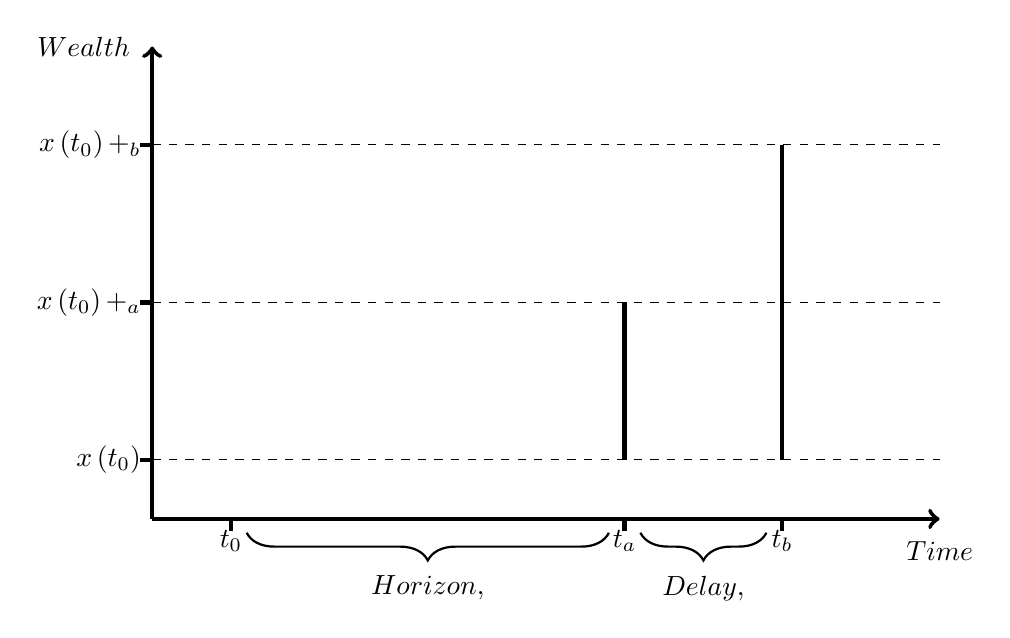
\begin{tikzpicture}
%\draw[help lines, color=gray!30, dashed] (-5,0) grid (4.9,5.9);
\draw[->,ultra thick] (-5,0)--(5,0) node[below,yshift=-4pt]{$Time$};
\draw[->,ultra thick] (-5,0)--(-5,6) node[left,xshift=-4pt]{$Wealth$};
\draw[-,ultra thick] (-4,-0.15)--(-4,0) node[below]{$t_0$};
\draw[-,ultra thick] (1,-0.15)--(1,0) node[below]{$t_a$};
\draw[-,ultra thick] (3,-0.15)--(3,0) node[below]{$t_b$};
\draw[-,ultra thick] (-5.15,0.75)--(-5,0.75) node[left]{$x\left(t_0\right)$};
\draw[-,ultra thick] (-5.15,2.75)--(-5,2.75) node[left]{$x\left(t_0\right) + \Dx_a$};
\draw[-,ultra thick] (-5.15,4.75)--(-5,4.75) node[left]{$x\left(t_0\right) + \Dx_b$};
\draw[-, dashed] (-5,0.75)--(5,0.75) ;
\draw[-, dashed] (-5,2.75)--(5,2.75) ;
\draw[-, dashed] (-5,4.75)--(5,4.75) ;
\draw[-, ultra thick] (1,0.75)--(1,2.75) ;
\draw[-, ultra thick] (3,0.75)--(3,4.75) ;
\draw [decorate,decoration={brace,amplitude=10pt,mirror},xshift=0pt,yshift=-5pt,thick](-3.8,0) -- (0.8,0) node [black,midway,yshift=-20pt]{$\text{Horizon, }\hor$};
\draw [decorate,decoration={brace,amplitude=10pt,mirror},xshift=0pt,yshift=-5pt,thick](1.2,0) -- (2.8,0) node [black,midway,yshift=-20pt]{$\text{Delay, }\del$};
\end{tikzpicture}
\caption{The basic setup of the model. A decision maker faces a choice at time $t_0$ between option $a$, which guarantees a payment of $\Dx_a$ at time $t_a$, and option $b$, which guarantees a payment of $\Dx_b>\Dx_a$ at time $t_b>t_a$. We define the time between the decision and the earlier payment as the {\it horizon}, $\hor\equiv t_a-t_0$; and the time between the two payments as the {\it delay}, $\del\equiv t_b-t_a$.}
\flabel{basicsetup}
\end{figure}

%\begin{figure}[!htb]
%\centering
%\includegraphics[width=0.4\textwidth]{./figures/setup.pdf}
%\caption{
%The basic setup of the model. A decision maker faces a choice at time $t_0$ between option $a$, which guarantees a payment of $\Dx_a$ at time $t_a$, and option $b$, which guarantees a payment of $\Dx_b>\Dx_a$ at time $t_b>t_a$.
%}
%\flabel{basicsetup}
%\end{figure}

We will describe four different specifications of this basic setup. In each we will calculate the growth rates, $g_a$ and $g_b$, of wealth associated with options $a$ and $b$.
%The decision maker prefers the option whose growth rate is larger.
From this analysis we will infer the discount function. This is the multiplicative factor, $\delta$, by which the later payment, $\Dx_b$, must be multiplied to equal the earlier payment, $\Dx_a$, when the payment amounts and times are such that the decision maker is indifferent between the two options ($\left(t_a,\Dx_a\right) \sim \left(t_b,\Dx_b\right)$). In symbols,

\be
\delta \equiv \left.\frac{\Dx_a}{\Dx_b}\right|_{g_a=g_b}\,,
\ee

\ie the ratio of payments under the constraint that the growth rates corresponding to $a$ and $b$ are equal.
%To calculate to DF, we evaluate the ratio between the payment $\Dx_a$ and the payment $\Dx_b$ under the assumption that the the growth rates $g_a$ and $g_b$ are equal.

As we show below, this setup predicts decisions equivalent to hyperbolic and exponential discounting under different specifications. Some specifications of the model predict preference reversal.
%Our model differs from many standard models in the literature by assuming that decision makers maximize the growth rate of their wealth, rather than the expected change in their utility.
%It has been shown to be equivalent in some cases, under specific dynamics and specific utility function choices~\citep{PetersAdamou2018a}. It is further discussed in~\Sref{discussion}.

\section{Results}\label{sec:results}

\subsection{Specification}

We begin by describing four different specifications for our basic setup. Each specifies two aspects necessary to quantify the growth rate of wealth: the time frame of the decision, and the dynamics under which wealth evolves.

The time frame is a key aspect, often left unspecified or implicit in similar setups in the literature~\citep{CohenETAL2019}. Consider the following scenarios:

\begin{enumerate}
\item Every January Bob the bureaucrat is given a budget. Bob must choose a project to fund with his allocated budget. All projects cost the entire allocated budget (there is no question of saving). He is paid upon the completion of each project.
%\item Dana, the developer, loves to work and always wants to keep busy with her development projects, she always gets paid at their completion. Dana has a choice between a project that lasts three months and a project that lasts six months, and she can only work on one project at a time.
\item Dana, the driver, has to decide whether to drive for Uber or for Bolt, two popular ride hailing services. While Uber rides pay her less than Bolt per ride, they are more abundant. She rarely has to wait for a new ride after completing one on Uber, while she usually has to wait for some time for a new ride to arrive on Bolt.
\end{enumerate}

In the first scenario, the important element to note is that no matter which choice is made, it will not affect the timing of future choices. Said otherwise, the time frame is independent of the choice, so we say it is {\it fixed}.%That is, the timing of Nate's next choice is not affected by his decision.
In the second scenario, the time frame depends on the choice made. That is, the timing of Dana's next choice is determined by her current decision. We call this the {\it adaptive} time frame.

%In the second scenario, the time frame depends on the choice made. We call this the {\it adaptive} time frame because Dana is more flexible to pursue other opportunities if she chooses the shorter project. On the other hand, if she chooses the longer project, it locks her in for a longer time period. This means we assume she will be able to make her next choice only after the longer project ends.

In our model, we must choose the time period over which the growth rates of wealth in each option are computed. We can choose it to be the time period associated with each payment, \ie $t_a-t_0$ for option $a$ and $t_b-t_0$ for option $b$. This specification corresponds to Dana's situation, the adaptive time frame specification. Or we can choose it always to be the longer time period, $t_b-t_0$, resembling Bob's dilemma, the fixed time specification.

%It should be noted that in the fixed time period there is also the question of overlapping projects. If the next choice occurs before the previous project has finished there is an implied multi-tasking capability that is not implied in the adaptive time frame. If the frequency of the budget is given by $t_f$ and the duration of projects is $t_a$, then the growth rate will fluctuate between $t_f g_a$ and $(t_f-1)g_a$ If an agent can only undertake a fixed number of projects, then if the overlap of the projects is frequent enough to exceed his multi-tasking capability then the growth rate $t_f g_a$ is not achievable. If the multi-tasking constrained binds, there needs to be a reformultation between variable and fixed?

%For convenience, we denote the two periods between the decision time and the known future payment times as $\Dt_a \equiv t_a-t_0$ and $\Dt_b \equiv t_b-t_0$. Additionally, we denote the known delay between the two payments as $D \equiv t_b-t_a$.


%\textcolor{red}{\begin{enumerate}
%\item A builder must choose between two jobs starting tomorrow, one paying \$1,000 for a week's work and the other paying \$3,000 for a month's work, with both sums being paid on completion of the work.
%\item An author must choose %between receiving \$30,000 in advance or \$50,000 on production of a book that will take a year to write.
%\end{enumerate}}

% \textcolor{red}{In the first scenario, the time frame depends on the choice made: one week for the smaller job; one month for the larger job. If the builder chooses the smaller job, he is free to pursue other opportunities during the three-and-a-bit weeks between its completion and the completion of the larger job. But if he chooses the larger job, he can do nothing else for the whole month. Although the guaranteed payment is greater, the larger job has an opportunity cost relative to the smaller one.}

%\textcolor{red}{In the second scenario, the time frame is independent of the choice: in both cases, the author must work for one year. In particular, taking the earlier payment does not allow her (ethically, at least) to pursue other opportunities during the period between it and the later payment that she declined.}


%\textcolor{red}{In our model, we must choose the time frame over which the growth rates of wealth in each option are computed. We can choose it to be the time period associated with each payment, \ie $\Dt_a$ for option $a$ and $\Dt_b$ for option $b$. This specification reminds us of the builder's choice and we will call it the adaptive time frame specification. Or we can choose it always to be the longer time period, $\Dt_b$, resembling the author's dilemma. We will call this the fixed time frame specification.}

%One possibility is to assume a fixed time frame -- the decision maker faces the choice every $\Dt_b$. In this case, in order to compare between the two choices, we will evaluate the growth rates between $t_0$ and $\Dt_b$ in both options. Another possible specification of time frame, is that the decision maker faces a choice after the payment is exercised, \ie after $\Dt_a$ if option $a$ was chosen and after $\Dt_b$ if option $b$ was chosen. In this case, we will evaluate the growth rate for option $a$ at time $\Dt_a$, and for option $b$ at $\Dt_b$. The former time frame will be labeled the fixed time frame and the latter the adaptive time frame.

As described in~\Sref{model}, the wealth dynamics can also take different forms, and we will address two specific common cases: additive and multiplicative wealth dynamics. We note that under the multiplicative dynamics it is assumed that the payment itself is re-invested at the risk-free rate. For additive dynamics there is essentially no re-investment of the payment -- income in this dynamic is independent of wealth.

We will discuss the four specifications, as illustrated in~\fref{tree}. In each case we will: compute the growth rates $g_a$ and $g_b$ associated with each option; compare them to determine the conditions under which each option is preferred; elicit the form of temporal discounting equivalent to our decision model; and, finally, determine whether preference reversal is predicted.

\begin{figure}[!htb]
\centering
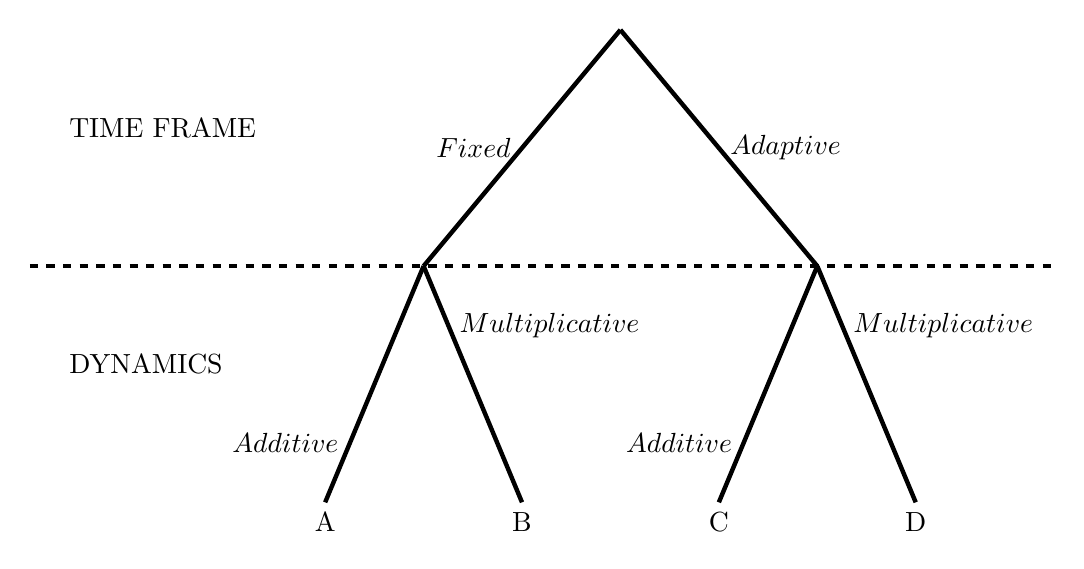
\begin{tikzpicture}
%\draw[help lines, color=gray!30, dashed] (-5,0) grid (4.9,5.9);
\draw[-,ultra thick] (0,6)--(-2.5,3) node[left,midway]{$Fixed$};
\draw[-,ultra thick] (0,6)--(2.5,3) node[right,midway]{$Adaptive$};
\node[text width=3cm] at (-5.5,4.75) {TIME FRAME};
\draw[-,ultra thick,dashed] (-7.5,3)--(5.5,3);
\draw[-,ultra thick] (-2.5,3)--(-3.75,0) node[left,near end]{$Additive$};
\draw[-,ultra thick] (-2.5,3)--(-1.25,0) node[right,near start]{$Multiplicative$};
\draw[-,ultra thick] (2.5,3)--(1.25,0) node[left,near end]{$Additive$};
\draw[-,ultra thick] (2.5,3)--(3.75,0) node[right,near start]{$Multiplicative$};
\node[text width=3cm] at (-5.5,1.75) {DYNAMICS};
\node at (-3.75,-0.25) {A};
\node at (-1.25,-0.25) {B};
\node at (1.25,-0.25) {C};
\node at (3.75,-0.25) {D};
\end{tikzpicture}
\caption{The four model specifications, determined by specifying a time frame and wealth dynamics. The labels A, B, C, and D, are used for the different cases.}
\flabel{tree}
\end{figure}

%\begin{figure}[!htb]
%\centering
%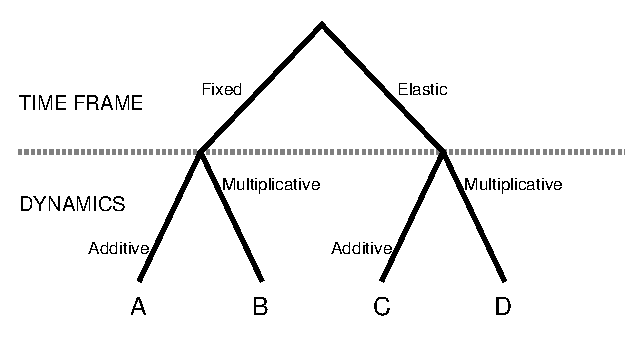
\includegraphics[width=0.5\textwidth]{./figures/tree2.eps}
%\caption{The four model specifications, determined by specifying a time frame and wealth dynamics. The labels A, B, C, and D, are used for the different cases.}
%\flabel{tree}
%\end{figure}

\subsection{Case A -- Fixed time frame with additive dynamics}\label{sec:case_C}

Specification: the period for computing the growth rate is that between the decision ($t_0$) and the later payment ($t_b$); and the wealth dynamics are additive. Here, regardless of the initial wealth and in addition to the chosen payment, wealth grows at an additive rate $k$ (corresponding to labor income, for example).

We begin by writing down the final wealth under each of the two options, evaluated at $t_b$:

\bea
x_a\left(t_b\right) &=& x\left(t_0\right) + k\left(t_b-t_0\right) + \Dx_a\,;\\
x_b\left(t_b\right) &=& x\left(t_0\right) + k\left(t_b-t_0\right) + \Dx_b\,.
\eea

The growth rates are:

\bea
g_a &=& \frac{x_a\left(t_b\right) - x\left(t_0\right)}{t_b-t_0} = \frac{\Dx_a}{t_b-t_0} + k\,;\\
g_b &=& \frac{x_b\left(t_b\right) - x\left(t_0\right)}{t_b-t_0} = \frac{\Dx_b}{t_b-t_0} + k\,.
\eea
%Note that the wealth and its growth rate under option $b$ are the same as in case A, since they were already evaluated at $t_b$.

We assume $\Dx_b > \Dx_a$, so option $b$ is always preferred to option $a$. This is a trivial case -- if we assume additive wealth dynamics and compare the growth rates at the same time (or assuming repetition over fixed periods), then only the payment size matters to the decision maker. In this case, the discount function $\delta$ cannot be defined since the later, larger payment is always preferred and the indifference condition is never satisfied.

\subsection{Case B -- Fixed time frame with multiplicative dynamics}\label{sec:case_D}

Specification: the period for computing the growth rate is that between the decision ($t_0$) and the later payment ($t_b$); and the wealth dynamics are multiplicative. This specification corresponds to the most standard case of temporal discounting -- wealth is continuously compounding at the risk-free rate, $r$, and payments are re-invested at this rate.

We note that in this case the earlier payment, $\Dx_a$, if chosen, is treated as growing exponentially from $t_a$ to $t_b$. The wealths evolve from $t_0$ to $t_b$ as follows:
\bea
x_a\left(t_b\right) &=& x\left(t_0\right) e^{r\left(t_b-t_0\right)} + \Dx_a e^{r\left(t_b-t_a\right)}\,;\\
x_b\left(t_b\right) &=& x\left(t_0\right) e^{r\left(t_b-t_0\right)} + \Dx_b\,.
\eea

The corresponding growth rates are:
\bea
g_a &= \frac{1}{t_b-t_0} \log{\left(\frac{x_a\left(t_b\right)}{x\left(t_0\right)}\right)} = \frac{1}{t_b-t_0}\log{\left(1 + \frac{\Dx_a e^{r\left(t_b-t_a\right)}}{x\left(t_0\right)e^{r\left(t_b-t_0\right)}}\right)} + r\,;\\
g_b &= \frac{1}{t_b-t_0} \log{\left(\frac{x_b\left(t_b\right)}{x\left(t_0\right)}\right)} = \frac{1}{t_b-t_0}\log{\left(1 + \frac{\Dx_b}{x\left(t_0\right)e^{r\left(t_b-t_0\right)}}\right)} + r\,.
\eea
%Note that the evolution of wealth under option $b$ is the same as in case B.

The criterion $g_a > g_b$ is simple, since only the numerator in the second term of the logarithm is different, so only this must be compared. Thus, $g_a > g_b$ if

\be
\Dx_a e^{r\left(t_b-t_a\right)} > \Dx_b\,.
\ee

We see that in this case the discount function depends on a single time periods -- that between the two payments, $t_b-t_a$, the delay $\del$. So the criterion $g_a > g_b$ in terms of the delay is

\be
\Dx_a e^{r\del} > \Dx_b\,.
\ee

The discount function is similarly expressed by setting the growth rates to be equal. Then we get $\Dx_a e^{r\del} = \Dx_b$ and

\be
\delta = \frac{\Dx_a}{\Dx_b} = e^{-r\del}\,,
\ee

which is the standard exponential discounting result~\citep{Samuelson1937}.\footnote{This result indeed corresponds to the historical use of the term ``rate of discount'', used to describe a risk-free interest rate in the money market (see, \eg~\citet{Jevons1863}).} The interpretation is straightforward: if it is possible to re-invest the earlier payment such that, by the time of the later payment, it will exceed the later payment amount, then option $a$ is preferred to option $b$ (and {\it vice versa}).

\subsection{Case C -- Adaptive time frame with additive dynamics}\label{sec:case_A}

Specification: the period for computing the growth rate is that between the decision ($t_0$) and the chosen payment; and the wealth dynamics are additive. Like in case A, regardless of the initial wealth and in addition to the chosen payment, wealth grows at an additive rate $k$ (corresponding to labor income, for example). Unlike case A, options $a$ and $b$ are evaluated at $t_a$ and $t_b$, respectively:

\bea
x_a\left(t_a\right) &=& x\left(t_0\right) + k\left(t_a-t_0\right) + \Dx_a\,;\\
x_b\left(t_b\right) &=& x\left(t_0\right) + k\left(t_b-t_0\right) + \Dx_b\,.
\eea

The growth rates are:

\bea
g_a &=& \frac{x_a\left(t_a\right) - x\left(t_0\right)}{t_a-t_0} = \frac{\Dx_a}{t_a-t_0} + k\,;\\
g_b &=& \frac{x_b\left(t_b\right) - x\left(t_0\right)}{t_b-t_0} = \frac{\Dx_b}{t_b-t_0} + k\,.
\eea

It follows that the criterion $g_a > g_b$ is

\be
\frac{\Dx_a}{t_a-t_0} > \frac{\Dx_b}{t_b-t_0}\,,
\ee

suggesting that under this specification only the linear payment rate of each option matters to the decision maker.

If we treat the payment amounts, $\Dx_a$ and $\Dx_b$, and payment times, $t_a$ and $t_b$, as fixed parameters of the problem, then we can elicit the dependence of the decision on the decision time, $t_0$. When both payments are far ahead in the future, the larger, later payment is preferred. In this case the ratio of the growth rates approaches $\lim_{t_0\to-\infty}\frac{g_a}{g_b}=\frac{\Dx_a}{\Dx_b}$, and $g_a<g_b$ since we have assumed $\Dx_a<\Dx_b$. When the earlier payment is imminent, \ie as $t_0\to t_a$, $g_a$ grows without bound while $g_b$ remains finite and so $g_a>g_b$. In other words, as time passes, our decision model predicts preference reversal from the later, larger payment to the earlier, smaller payment, under this specification. This is illustrated in~\fref{caseC}.

\begin{figure}[!htb]
\centering
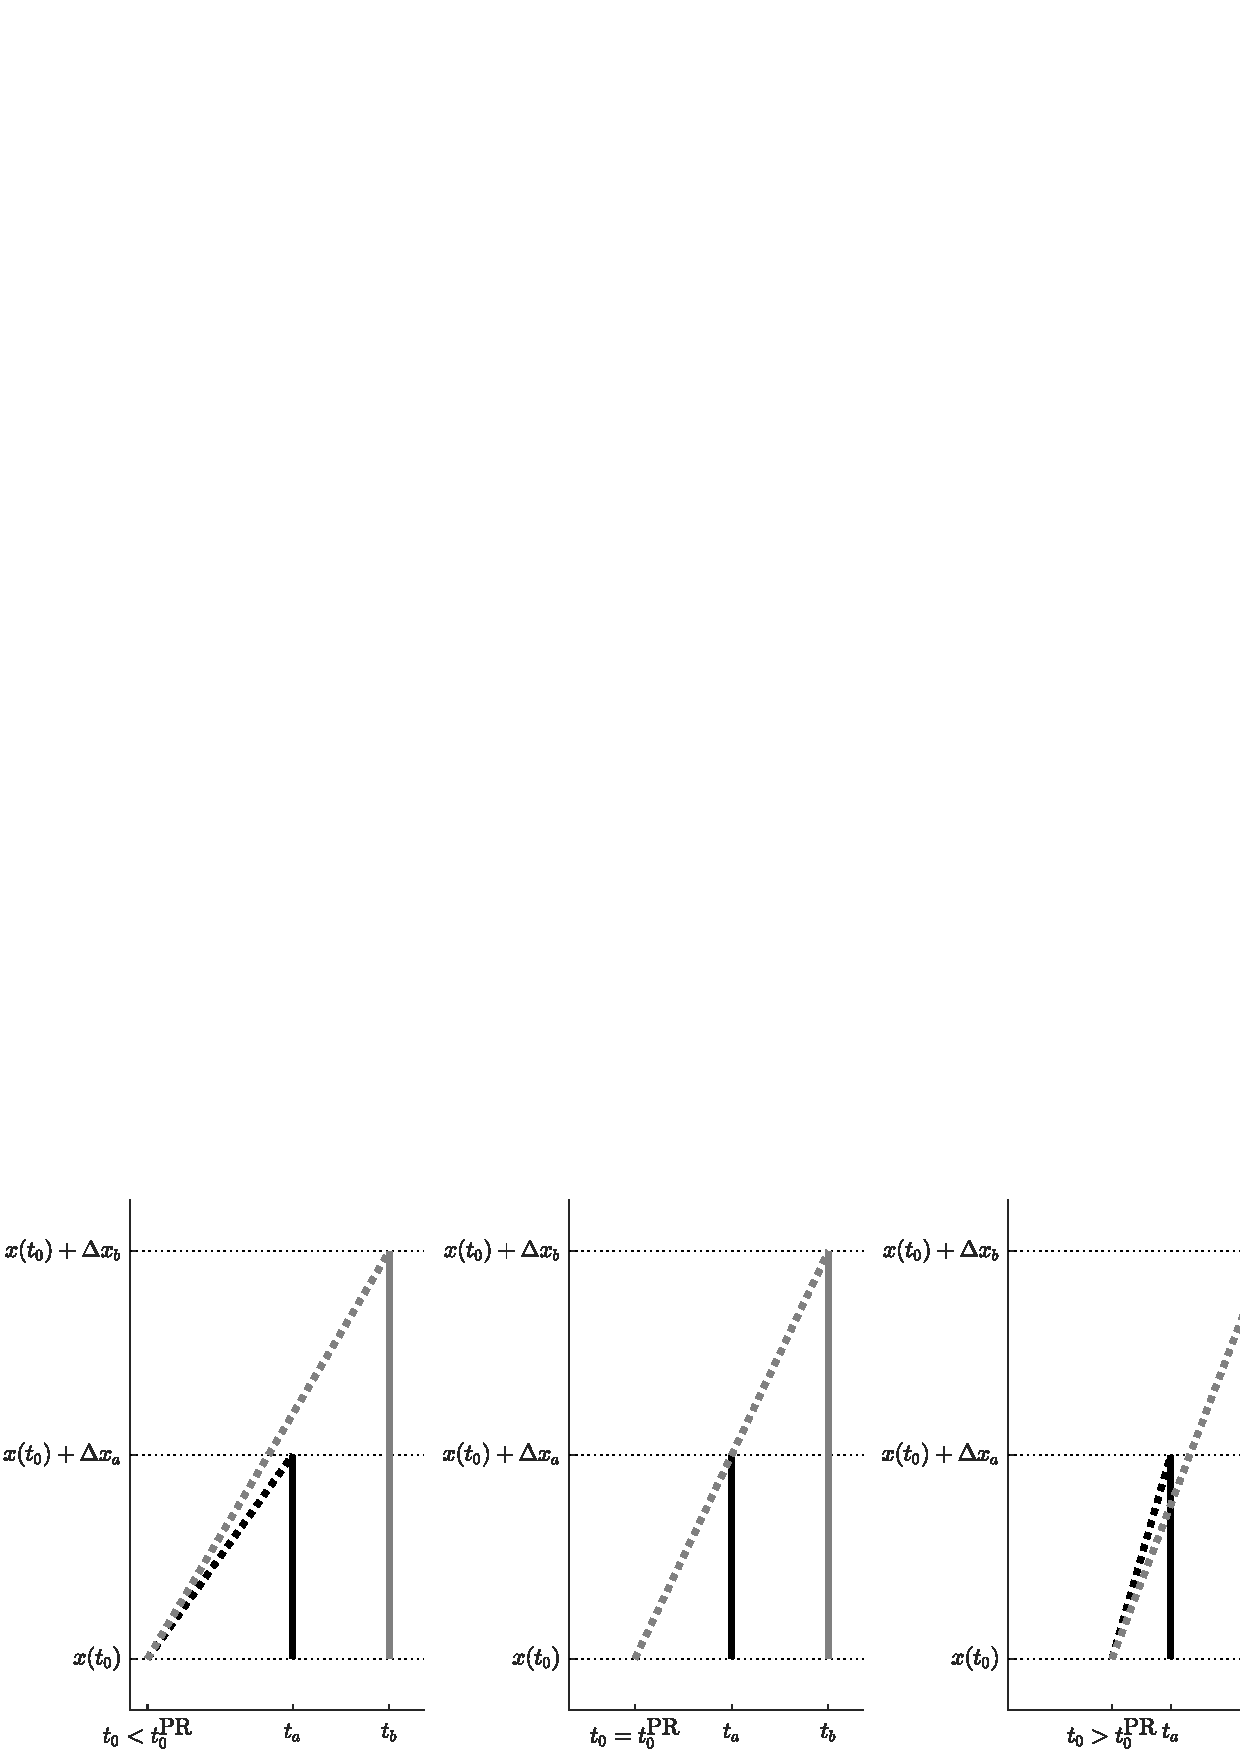
\includegraphics[width=1.0\textwidth]{./figures/caseC_reversal.jpg}
\caption{Preference reversal in case C. From left to right panel, $t_0$ increases, that is, the time of the payments approaches, while all other parameters are unchanged. Initially, option $b$ is preferred, having the higher growth rate. At a later time $t_0=t_0^\text{PR}$, given by~\eref{t0PR}, both options imply equal growth, and preference reversal occurs. At later times option $a$ is preferred.}
\flabel{caseC}
\end{figure}

%\begin{figure}
%\centering
%\begin{picture}(420,100)(0,0)
%\put(-50,0){\includegraphics[width=0.39\textwidth]{./figures/reversal_1.pdf}}
%\put(110,0){\includegraphics[width=0.39\textwidth]{./figures/reversal_2.pdf}}
%\put(270,0){\includegraphics[width=0.39\textwidth]{./figures/reversal_3.pdf}}
%\end{picture}
%\caption{
%Preference reversal in case A. From left to right panel, $t_0$ increases, that is, the time of the payments approaches, while all other parameters are unchanged. Initially, option $b$ is preferable, having the higher growth rate. At a later time $t_0=t_0^{PR}$, given by \eref{t0PR}, both options imply equal growth, and preference reversal occurs. At later times option $a$ is preferable. 
%}
%\flabel{caseA}
%\end{figure}

%It shows that the payment rate of option $b$ is higher than that of option $a$, which makes it preferable. This holds for some time. However, at some point in time, this changes and the payment rate of option $a$ would be higher. Assuming that initially option $g_b > g_a$, there will always be a point in time in which PR will occur. If time $\tau$ elapsed from $t_0$, than the updated payment rates of options $a$ and $b$ are $\frac{\Dx_a}{\Dt_a - \tau}$ and $\frac{\Dx_b}{\Dt_b - \tau}$, respectively. The reversal will occur when these are equal, or
%\be
%\tau_{\text{reversal}} = \frac{\Dt_a\Dx_b - \Dt_b\Dx_a}{\Dx_b - \Dx_a}\,.
%\ee

We can compute the decision time, $t_0^\text{PR}$, at which preference reversal occurs by setting $g_a=g_b$ to give
\be
t_0^\text{PR} = \frac{\Dx_b t_a - \Dx_a t_b}{\Dx_b - \Dx_a}.
\elabel{t0PR}
\ee

We can also find the discount function under this specification. When $g_a=g_b$, we have
\be
\delta = \frac{\Dx_a}{\Dx_b} = \frac{t_a-t_0}{t_b-t_0} = \frac{1}{1+\frac{t_b-t_a}{t_a-t_0}} = \frac{1}{1+\del/\hor}\,,
\ee

where we have made the final manipulation to express $\delta$ in hyperbolic form.

In this case the discount function depends on both the horizon and the delay.\footnote{Indeed, the problem is fully specified by these two time periods and the two payment amounts. The actual times, $t_0$, $t_a$, $t_b$, are not needed to specify the problem because, when computing growth rates, only elapsed times matter. The time origin is arbitrary. Also, for this reason, $t_0^\text{PR}$, the preference reversal time in case C, can be negative if option $b$ is already preferred to option $a$ at the time of decision, $t_0$.} The discount function is thus a hyperbolic function of the delay $\del$. The degree of discounting parameter used in many models (see, \eg~\citet{LoewensteinPrelec1992,Laibson1997}) is replaced here by $1/\hor$, the reciprocal of the horizon. As the horizon gets shorter, $1/\hor$ becomes larger, $\delta$ gets smaller, and the later payment becomes less favorable. No knowledge of the decision maker's psychology is required in this setup -- only the postulate that she prefers her wealth to grow faster rather than slower.

%The discount factor, $\delta$, is the factor by which the later payment, $\Dx_b$, must be multiplied to equal the earlier payment, $\Dx_a$, under indifference between options $a$ and $b$. Practically, it can be found by considering the equality of growth rates $g_a$ and $g_b$, which is the condition for indifference. $\delta$ is typically presented as a function of the time difference between options. In our setup this would be $\Epsilon \equiv \Dt_b - \Dt_a$.
%
%\textcolor{red}{
%Now that we have the hyperbolic DF in terms of the delay, $\Dt_b-\Dt_a$, and the time to the first payment, $\Dt_a$, as
%\be
%\delta = \frac{1}{1+\frac{\Dt_b-\Dt_a}{\Dt_a}} = \frac{1}{1+kD},
%\ee
%it would be much clearer to present PR as a consequence of changing the time to the first payment rather than the reference time. Then $t_0\to t_0+\Dt_a$ is simply $\Dt_a\to0$, which is also expressible as $k\to\infty$. This minor reframing will require some changes below, including to the figure, because we would treat $t_0$ as fixed and $\Dt_a$ as movable.
%}
%\textcolor{red}{
%Do we need $\Epsilon$? The letter has no intuitive meaning (to me) and perhaps we can get away without relabelling $\Dt_b-\Dt_a$. If not, $D$ for delay or $W$ for wait might be better.
%}
%XXXOP: not sure -- I like the physical time $t_0$ changing. What happens in real life is that time ticks on and we get swept towards $t_a$, it's not that we sit still in time, and someone tunes $t_a$. Agree about $\Epsilon$ -- better letter?XXX
%
%
%In case A we therefore get
%\be
%\delta_A = \frac{\Dx_a}{\Dx_b} = \frac{\Dt_a}{\Dt_b} = \frac{1}{1+\frac{1}{\Dt_a} \Epsilon}\,.
%\ee
%
%This is exactly hyperbolic discounting with degree of discounting $\kappa = \frac{1}{\Dt_a}$.

Finally, we note that $k$, the background growth rate of the decision maker's wealth, does not appear in the decision criterion. This is because wealth growth is not affected by exogenous cash flows under additive dynamics: the gain $k\Dt$ over period $\Dt$ occurs regardless of other payments received. This contrasts with multiplicative dynamics, where payments can be subjected to the growth process through re-investment.

\subsection{Case D -- Adaptive time frame with multiplicative dynamics}\label{sec:case_B}

Specification: the period for computing the growth rate is that between the decision ($t_0$) and the chosen payment; and the wealth dynamics are multiplicative, with rate $r$.

We follow the same steps as in the previous cases. Wealth evolves to:

\bea
x_a\left(t_a\right) &=& x\left(t_0\right) e^{r\left(t_a-t_0\right)} + \Dx_a\,;\\
x_b\left(t_b\right) &=& x\left(t_0\right) e^{r\left(t_b-t_0\right)} + \Dx_b\,.
\eea

The corresponding growth rates are:

\bea
g_a &= \frac{1}{t_a-t_0} \log{\left(\frac{x_a\left(t_a\right)}{x\left(t_0\right)}\right)} = \frac{1}{t_a-t_0}\log{\left(1 + \frac{\Dx_a}{x\left(t_0\right)e^{r\left(t_a-t_0\right)}}\right)} + r \elabel{ga_B}\,;\\
g_b &= \frac{1}{t_b-t_0} \log{\left(\frac{x_b\left(t_b\right)}{x\left(t_0\right)}\right)} = \frac{1}{t_b-t_0}\log{\left(1 + \frac{\Dx_b}{x\left(t_0\right)e^{r\left(t_b-t_0\right)}}\right)} + r\,.\elabel{gb_B}
\eea

This setting displays preference reversal: $g_a<g_b$ for $t_0$ sufficiently far away from $t_a$ (long horizon); and $g_a>g_b$ for $t_0$ sufficiently close to $t_a$ (short horizon). No closed-form expression for the reversal time, $t_0^\text{PR}$, is available. Similarly, the discount function $\delta$ cannot be derived explicitly.

Case D also displays another type of preference reversal under some conditions. Varying initial wealth $x\left(t_0\right)$ while keeping all other parameters fixed can lead to a switch from $g_a>g_b$ to $g_a<g_b$, as illustrated in~\fref{reversal_B}.
%An example is given in panel A of \fref{reversal_2}, and 

\begin{figure}[!htb]
\centering
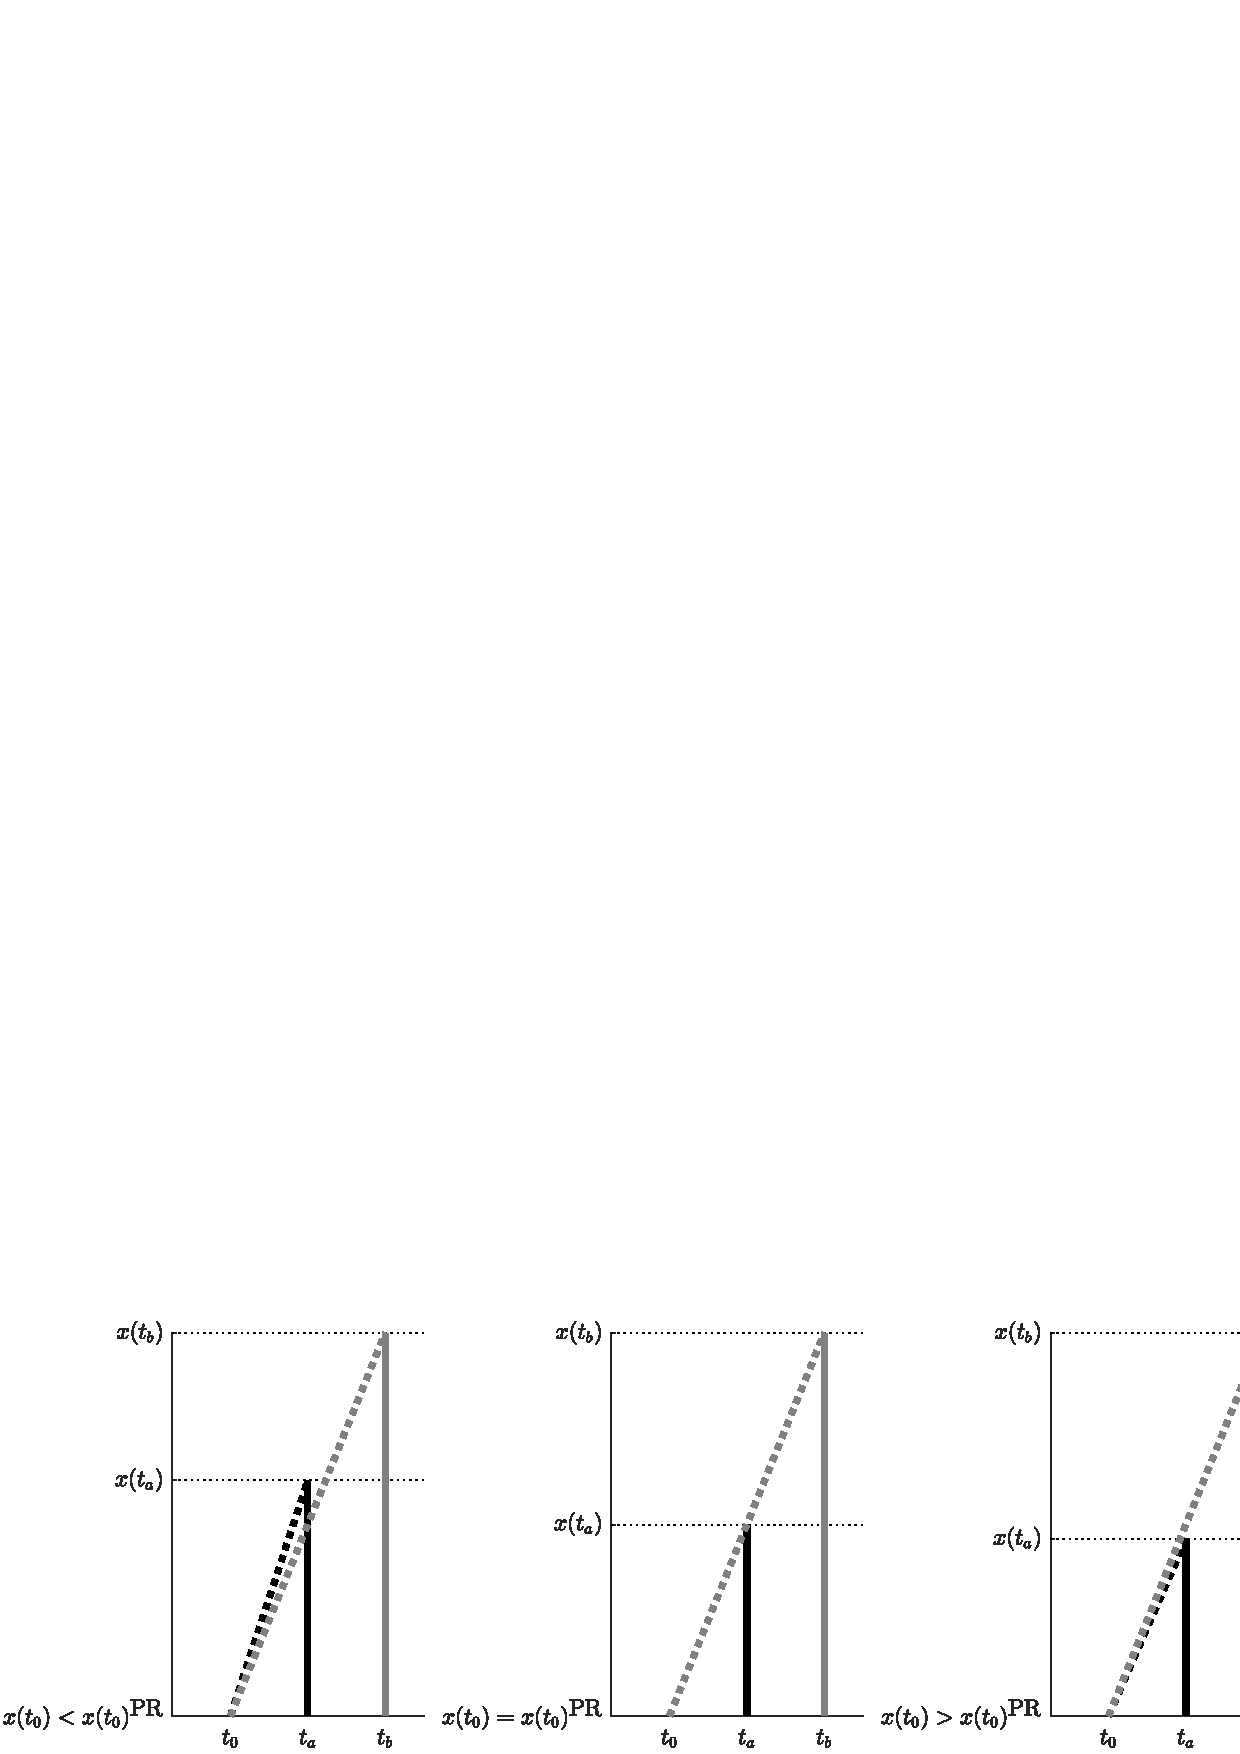
\includegraphics[width=1.0\textwidth]{./figures/caseD_reversal.jpg}
\caption{Preference reversal in response to wealth changes, in case D, logarithmic vertical scales. Initial wealth $x\left(t_0\right)$ increases from left to right panel (\$500, \$2277, \$5500), while all other parameters are unchanged ($t_0=$ today, $t_a=1$~year from today, $t_b=2$~years from today, $\Dx_a=\$1000$, $\Dx_b=\$2500$, $r=0.03$~per annum). At low wealth, option $a$ is preferred, having the higher growth rate, according to~\eref{ga_B} and~\eref{gb_B}. At a greater wealth, $x\left(t_0\right)^{PR}\approx \$2277$, both options imply equal growth, and preference reversal occurs. At even greater wealth, option $b$ is preferred: the poor behave optimally by choosing the earlier, smaller payment.}
\flabel{reversal_B}
\end{figure}

%\begin{figure}
%\centering
%\begin{picture}(420,100)(0,0)
%\put(-50,0){\includegraphics[width=0.39\textwidth]{./figures/reversal_B_1.pdf}}
%\put(110,0){\includegraphics[width=0.39\textwidth]{./figures/reversal_B_2.pdf}}
%\put(270,0){\includegraphics[width=0.39\textwidth]{./figures/reversal_B_3.pdf}}
%\end{picture}
%\caption{
%Preference reversal in response to wealth changes, in case B, logarithmic vertical scales. Initial wealth $x(t_0)$ increases from left to right panel (\$500, \$2277, \$5,000), while all other parameters are unchanged ($t_0=$ today, $t_a=1$~year from today, $t_b=2$~years from today, $\Dx_a=\$1000$, $\Dx_b=\$2500$, $r=0.03$~per annum). At low wealth, option $a$ is preferable, having the higher growth rate, according to \eref{ga_B} and \eref{gb_B}. At a greater wealth, $x(t_0)^{PR}\approx \$2277$, both options imply equal growth, and preference reversal occurs. At even greater wealth, option $b$ is preferable: the poor behave optimally by choosing the small early payment.
%}
%\flabel{reversal_B}
%\end{figure}

This type of reversal is further illustrated in the following example, with the same parameters used in~\fref{reversal_B}: Suppose an agent faces a choice between receiving $\$1000$ after 1 year (option $a$) or $\$2500$ after two years (option $b$), and we assume the agent has access to a risk-free interest rate of 0.03 per annum. If the agent has initially $\$500$, she will evaluate that the growth rate corresponding to option $a$ as

\be
g_a = \frac{1}{1}\log{\left(1 + \frac{1000}{500e^{0.03\cdot 1}}\right)} + 0.03 \approx 1.1\text{~per annum}\,,
\ee

and to option $b$ as

\be
g_b = \frac{1}{2}\log{\left(1 + \frac{2500}{500e^{0.03\cdot 2}}\right)} + 0.03 \approx 0.9\text{~per annum}\,.
\ee

Thus, the agent would prefer the earlier, smaller payment, as $1.1 > 0.9$. If we assume that the agent had initially $\$5500$, \ie, 11 times more than in the previous setting, a similar calculation yields $g_a\approx0.19$ and $g_b\approx0.21$, so the later, larger payment is preferred.% This means that a poorer individual would prefer the earlier choice.

The difference $g_a-g_b$, from~\eref{ga_B} and~\eref{gb_B}, is shown as a function of $x\left(t_0\right)$ in~\fref{reversal_B2}. This type of preference reversal can be expressed as follows: assuming multiplicative dynamics and an adaptive time frame, it is growth-optimal for people of lower wealth to choose an earlier, smaller payment, whereas it is growth-optimal for wealthier individuals to hold out until the later, larger payment. This predicts the findings of~\citet{EpperETAL2018}, that ``individuals with relatively low time discounting are consistently positioned higher in the wealth distribution'', and is likely consistent with~\citet{GreenETAL1996}, who found that people with higher incomes discount less steeply.

\begin{figure}[!htb]
\centering
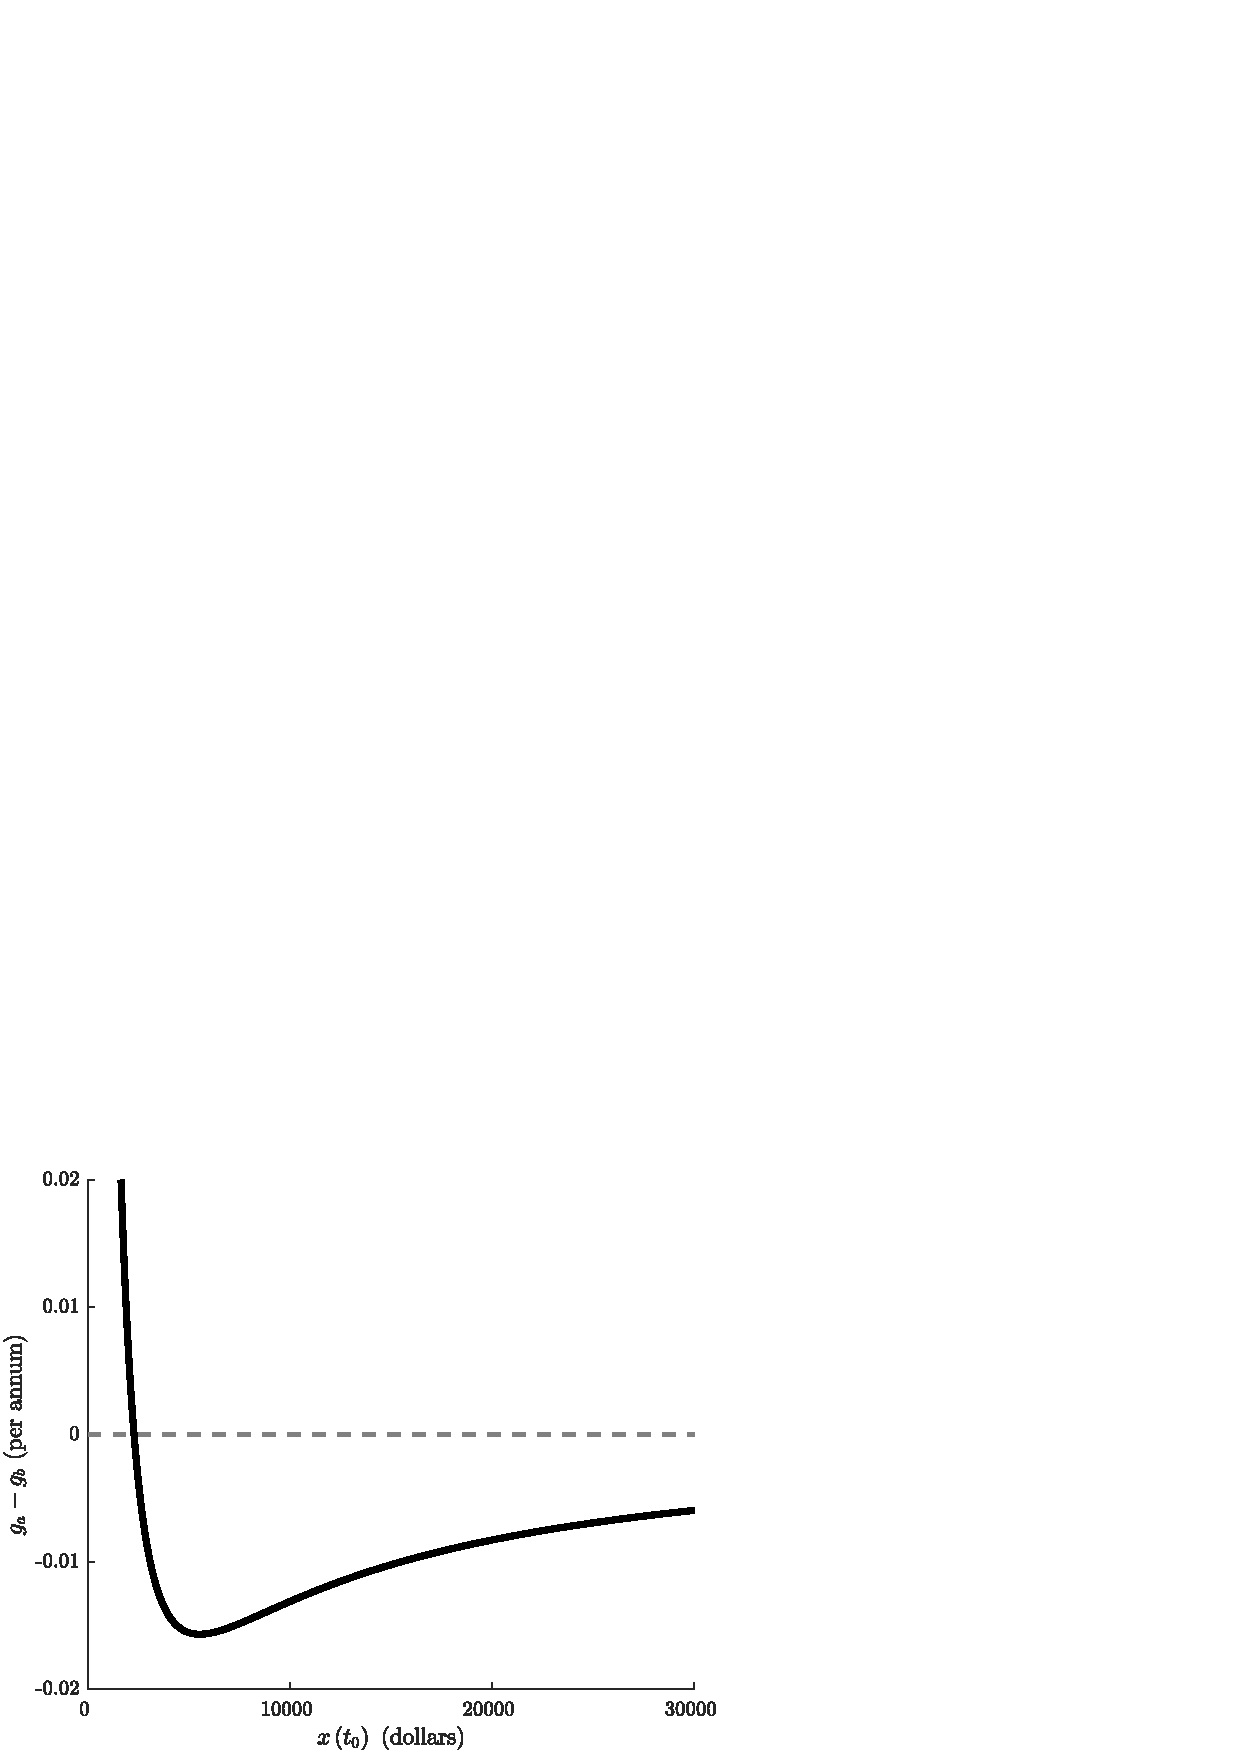
\includegraphics[width=0.7\textwidth]{./figures/caseD_ga_gb.jpg}
\caption{The difference $g_a-g_b$ as a function of the wealth at the time of decision ($x\left(t_0\right)$) in case D. The difference is positive when the earlier payment is preferred, and otherwise negative. We see that for small initial wealths $x\left(t_0\right)$ the earlier, smaller payment is preferred, whereas for large initial wealth the later, larger payment is preferred (parameters as used in~\fref{reversal_B}).}
\flabel{reversal_B2}
\end{figure}

We note that this kind of preference reversal is not predicted if $\Dx_b$ is not sufficiently large or if the delay is too long. In the limit $x\left(t_0\right)\to \infty$, we get

\be
g_a - g_b \approx \frac{1}{x\left(t_0\right)} \left(\frac{\Dx_a}{He^{rH}} - \frac{\Dx_b}{\left(H+D\right)e^{r\left(H+D\right)}}\right)\,.
\ee

Thus, option $b$ will preferred to option $a$ in this limit only if

\be
\Dx_b > \frac{\left(H+D\right)e^{r\left(H+D\right)}}{He^{rH}}\Dx_a\,.
\ee

Otherwise, the earlier, smaller payment is preferred for all wealth levels.

\subsubsection{Discounting in the small payment limit}

In many applications of discounting, it is plausible to assume that the payments are small relative to wealth:

\bea
\Dx_a \ll x\left(t_0\right)e^{r\left(t_a-t_0\right)}\,;\\
\Dx_b \ll x\left(t_0\right)e^{r\left(t_b-t_0\right)}\,.
\eea

In case D, it is possible to derive an approximated discount function in this limit. Setting $g_a=g_b$ and using the first-order approximation $\log(1+\epsilon)\approx\epsilon$ for $\epsilon\ll1$, we get

\be
\delta = \frac{\Dx_a}{\Dx_b} \approx \frac{\left(t_a-t_0\right)e^{r\left(t_a-t_0\right)}}{\left(t_b-t_0\right)e^{r\left(t_b-t_0\right)}} = \frac{e^{r\left(t_a-t_b\right)}}{1+\frac{t_b-t_a}{t_a-t_0}}\,.
\ee

Using the previous definitions of $\hor$ and $\del$, we can write this as

\be
\delta \approx \frac{e^{-r\del}}{1+\del/\hor}\,.
\ee

This is a hybrid case of hyperbolic and exponential discounting. It displays an interesting asymptotic behavior. For short delays a decision maker will discount hyperbolically. For long delays discounting will be approximately exponential, as illustrated in~\fref{shortpaymentasymp}. Thus, for the same dynamic and the same time frame, and assuming small payments relative to initial wealth, our choice axiom predicts both hyperbolic and exponential discount functions, only by changes in the delay between the two payments. We note again that only the elapsed times, $\hor$ and $\del$, appear in the discount function. However, the background wealth growth rate, $r$, no longer cancels out when dynamics are multiplicative, as does $k$ when they are additive. This result gives a quantitative and falsifiable prediction of the circumstances under which one could expect to observe either hyperbolic or exponential discounting in the same setup.

\begin{figure}[!htb]
\centering
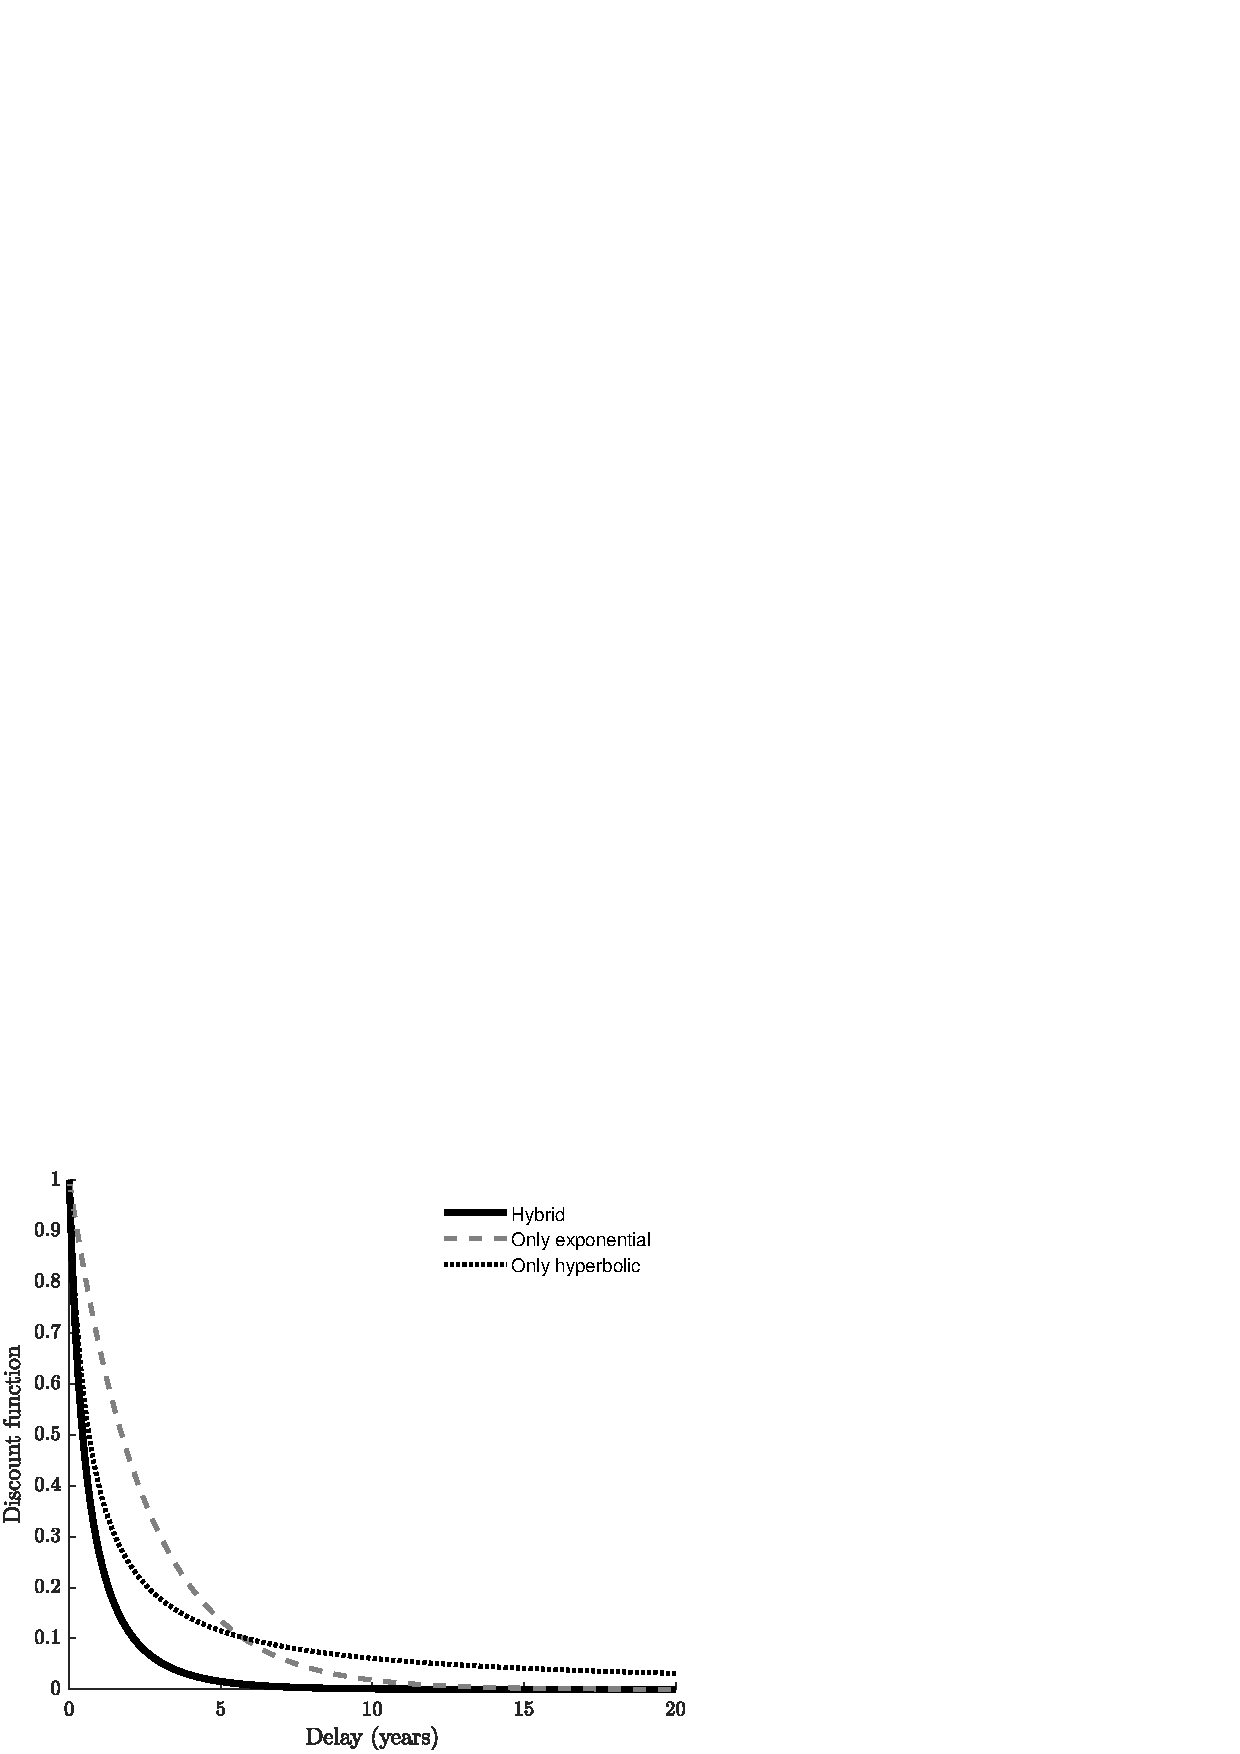
\includegraphics[width=0.7\textwidth]{./figures/caseD_delta_asymptotic.jpg}
\caption{The dependence of the discount function on the delay in the small payment limit. The solid black curve is the hybrid $\delta = \frac{e^{-r\del}}{1+\del/\hor}$, for $r=0.4\text{ per annum}$ and $\hor=0.65\text{ years}$. The discount function follows the hyperbolic discount function $\frac{1}{1+\del/\hor}$ for short delays. For long delays it asymptotically follows the exponential discount function $e^{-r\del}$.}
\flabel{shortpaymentasymp}
\end{figure}

\section{Conclusion}\label{sec:discussion}

This paper describes a model of discounting in a basic temporal choice problem. In this problem a decision maker must choose between two known, certain, and different payments to be made at known, certain, and different future times. We assume that a decision is made by comparing the growth rate of wealth associated with each option. We then study temporal discounting that results from this decision criterion, while specifying it fully by introducing: the wealth dynamics, treating specifically additive and multiplicative cases; and the time frame of the decision, meaning the period over which it is appropriate to compute growth rates.

Depending on the specification, our model predicts four different forms of discounting: no discounting; exponential; hyperbolic; and a hybrid of exponential and hyperbolic. This is not an exhaustive list -- other dynamics would produce other forms of discounting. Two of the discount functions nested in our model (hyperbolic and hybrid) are compatible with conventional preference reversal. One (hybrid) predicts another type of preference reversal, in which the decision maker switches from earlier to later payment as their resources increase. Thus, the model predicts richer people would discount less steeply under multiplicative dynamics and an adaptive time frame. This is inline with empirical findings~\citep{GreenETAL1996,EpperETAL2018}.

A major result of our model is that it predicts exponential and non-exponential discounting, as well as preference reversal, from theoretical considerations that do not violate standard axioms of choice~\citep{vonNeumannMorgenstern1944}. The model assumes no bias in the decision maker's behavior. Thus, if corroborated empirically, it would be both normative and descriptive. In particular, the model assumes no dynamic inconsistency in that the decision maker prefers at all times the option with the highest growth rate.
%A major conclusion is that discounting can be simply interpreted as growth rate optimization. We find that depending on the wealth dynamics assumed by the decision maker, growth rate optimization can be equivalent to hyperbolic discounting.

The cases studied are all riskless. A natural extension of this paper, planned for future work, is the inclusion of risk. In the presence of risk, the model will still assume that the maximand is the growth rate of wealth/resource over time. The risk will be embedded in time -- higher risk will tend to decrease the growth rate associated with a specific option~\citep{PetersGell-Mann2016}, making it less desirable. Such a framework is still based on a single axiom -- a decision maker prefers her wealth to grow faster than slower. No other assumptions on the risk preferences of the decision maker will be needed.

We note that the dynamics discussed here do not cover the entire range of possible dynamics. Although multiplicative and additive wealth dynamics are very common, and also simple and intuitive, it is possible that other wealth dynamics are relevant in some applications. While different dynamics require different calculation of growth rates, our model prediction is still that choices are made so that growth rates are maximized. Thus, generalizing the model results to other dynamics is straightforward (see~\citet{PetersGell-Mann2016,PetersAdamou2018a}).

We also note that the fixed and adaptive time frames do not cover all possible time frames. In reality, time frames may overlap, \ie it is possible for a decision maker to decide on future payments before an anticipated payment has been paid already. For example, a manager makes a decision about a project, but before the chosen project is done and a payment received, a decision about other future projects is made. We leave the treatment of such cases for future work.

We wish to emphasize that no knowledge of the decision maker's psychology is required in our setup -- only the postulate that she prefers her wealth to grow faster rather than slower. This postulate is enough for predicting a decision maker's discount functions used in standard discounted utility models. Yet, we also note that this paper discusses discounting from a theoretical perspective. An important complementary step of this research would be comparing the theoretical predictions of the results to empirical and experimental results. In particular, the predicted discount functions can be compared to results from controlled experiments. This is also planned for future work.

%We emphasize that our model is applied to a temporal choice between two {\it future} payments. Its applicability breaks down when the horizon goes to zero. In the limit $H\rightarrow0$, the growth rate corresponding to the earlier payment in cases C and D will go to infinity. This amounts to assuming the earlier payment is repeated indefinitely in an unrealistically high frequency, as our model relies on the argument that ``the discounting process used for the one-off events seems to obey a law that evolved as an adaptation to cope with repetitive events.''~\citep{Kacelnik1997}

We emphasize that our model is applied to a temporal choice between two {\it future} payments. In the small horizon limit, $H \to 0$, the growth rates corresponding to the earlier payment in cases C and D diverge, indicating a loss of realism. Here we can link it to the break down of an assumption. It is implicit in our model that the growth rates we compute are sustained over sufficiently long times to be meaningful maximands to the decision maker. They are, in effect, the growth rates of wealth achieved under repetition of the choice. We share the view of~\citet[p.~60]{Kacelnik1997} that ``the discounting process used for the one-off events seems to obey a law that evolved as an adaptation to cope with repetitive events.'' As the horizon shrinks, this repetition occurs at a frequency so high that the choice problem can no longer reflect reality.
%Receiving a payment by the end of this sentence is unlikely to mean a second payment at the end of the next.
